\begin{frame}{\LaTeX-Geschichte}
\begin{figure}[htbp]
\centering
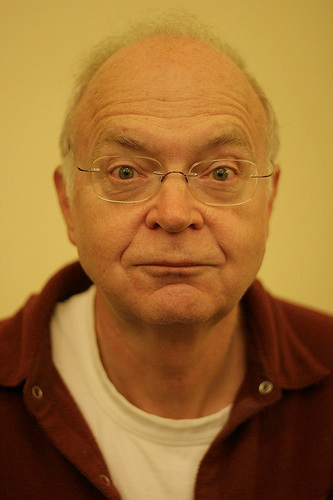
\includegraphics[width=\textwidth*0.8,height=\textheight*0.8,keepaspectratio]{../img/knuth.jpg}
\caption{Donald E. Knuth}
\end{figure}

\end{frame}

\begin{frame}{Donald E. Knuth}

\begin{itemize}
\itemsep1pt\parskip0pt\parsep0pt
\item
  emeritierter Professor (Stanford)
\item
  fast jährliche Preise und Auszeichnungen seit 1970 bis heute
\item
  25 Ehrendoktortitel
\item
  Knuth-Preis: außergewöhnliche Leistungen in den Grundlagen der
  Informatik
\item
  Asteroid: (21656) Knuth
\end{itemize}

\end{frame}

\begin{frame}{Trivia?}

\begin{itemize}
\itemsep1pt\parskip0pt\parsep0pt
\item
  ab 1. Januar 1990: mehr Konzentration auf Arbeit, nutzt keine E-Mails
  mehr
\item
  Korrektheit ist sehr wichtig: verschickt Schecks über 2.56\$ für
  gefundene Fehler
\item
  (wg. der Angst vor Scheckbetrug benutzt er nun die digitale Währung
  einer fiktiven Bank, zahlt das Guthaben aber auch gerne aus)
\end{itemize}

\end{frame}

\begin{frame}{verstehen Sie Spaß?}

\begin{figure}[htbp]
\centering
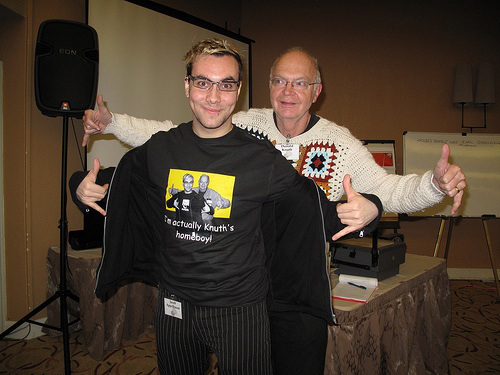
\includegraphics[width=\textwidth*0.8,height=\textheight*0.8,keepaspectratio]{../img/knuth-applebaum.jpg}
\caption{mit Jacob Applebaum}
\end{figure}

\end{frame}

\begin{frame}{Ein Buch über Comiler}

\begin{itemize}
\itemsep1pt\parskip0pt\parsep0pt
\item
    Knuth (noch Student im Hauptstudium) schreibt ein Buch über Compiler
\item
    \textit{Do you mind if I make this book a little bit longer, because I think there's a need for explaining these things in somewhat more detail.}
\item
    \textit{They said, ‚Oh no, go right ahead. Make it as long as you feel necessary.'}
\item
  Ergebnis: 3900 Seiten (1968)
\end{itemize}

\end{frame}

\begin{frame}{The Art of Computer Programming}

\begin{itemize}
\itemsep1pt\parskip0pt\parsep0pt
\item
  Band 1: 1968, Band 5 (von 7): 2020
\item
  legendäres Grundlagenwerk
\item
  eigener theoretischer, idealer Computer MIX, eigene Assemblersprache
  MIXAL
\item
  Themen: Algorithmen und Datenstrukturen (und Zahlentheorie, Suchen,
  Sortieren, uvm.)
\end{itemize}

\end{frame}

\begin{frame}{\TeX \ entsteht}

\begin{itemize}
\itemsep1pt\parskip0pt\parsep0pt
\item
  Überarbeitung von Band 2: Knuth erfindet \TeX
\item
  Schriftartendesign, Satztechnik, \ldots{}
\item
  Bücher über \TeX \ in \TeX: Spezifikation und Benutzung
\item
  Erklärung von Verfahren, z.B.: Worttrennungsalgorithmus
\end{itemize}

\end{frame}

\begin{frame}{\LaTeX \ und \LaTeXe}

\begin{itemize}
\itemsep1pt\parskip0pt\parsep0pt
\item
  1980: Leslie \emph{La}mport entwickelt Makros für \TeX: \emph{La}TeX
\item
  1990: Lamport beendet die Entwicklung. \LaTeX \ wird fortgeführt.
\item
  1994: \LaTeXe ist die Fortführung von \LaTeX
\item
  bedeutet: \LaTeX \ ist älter als Unicode
\end{itemize}

\end{frame}

\begin{frame}{Exkurs: Unicode}

\begin{itemize}
\itemsep1pt\parskip0pt\parsep0pt
\item
  internationaler Standard zur Zeichenkodierung (Version 1.0.0: Oktober
  1991)
\item
  soll \emph{jedes} sinntragende Zeichen umfassen
\item
  alle bekannten Schriftkulturen und Zeichensysteme
\item
  ein Beispiel für einen Codepunkt: \texttt{U+1F600} (welcher ist das?)
\item
  UTF-8: 8-bit Kodierung für Unicode-Zeichen, sehr verbreitet
\item
  Internet Engineering Task Force: neue Protokolle müssen UTF-8 können
\end{itemize}

\end{frame}

\begin{frame}{Aufgaben}

\begin{itemize}
\itemsep1pt\parskip0pt\parsep0pt
\item
  mit dem Hintergrund von \LaTeX \ und Unicode-Wissen, versuchen Sie
  folgendes herauszufinden:
\item
  was ist pdfTeX?
\item
  was ist \XeTeX? Inwiefern ist \XeTeX \ besser als \LaTeX?
\item
  was ist \LuaTeX? Was macht \LuaTeX \ anders als pdfTeX?
\end{itemize}

\end{frame}
